\documentclass[12pt, twoside]{report}
\usepackage[a4paper,bindingoffset=0.2in,%
    left=0.8in,right=0.8in,top=1.2in,bottom=1.2in,%
]{geometry}
\usepackage{graphicx}
\usepackage{fancyhdr}
\usepackage{comment}
\fancyhf{}
\renewcommand{\headrulewidth}{0pt}
\fancyhead[RO,LE]{\thepage}
\pagestyle{fancy}

\begin{document}

Saket:- Add Page 5-6

\subsection*{Prototypic Emotional Expressions}
Instead of describing the detailed facial features, most FER systems attempt to recognize a small set of prototypic emotional expressions. The most widely-used set is perhaps human universal facial expressions of emotion which consists of six basic expression categories that have been shown to be recognizable across cultures \ref{fig:facialPhenotypes} .

These expressions, or facial configurations have been recognized in people from widely divergent cultural and social backgrounds, and they have been observed even in the faces of individuals born deaf and blind.

These 6 basic emotions, \textit{i.e.}, disgust, fear, joy, surprise, sadness and anger plus ``neutral'' which means no facial expression are considered in this work. Given a facial image, our system either works as a conventional classifier to determine the most likely emotion or estimates the weights (or possibility) of each emotion as a fuzzy classifier does.

\begin{figure}[h]
    \centering
    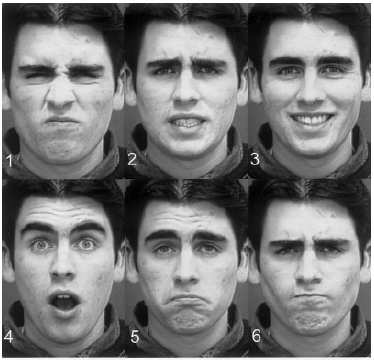
\includegraphics[width=0.5\textwidth]{img/7_1.png}
    \caption{Basic facial expression phenotypes. 1, disgust; 2, fear; 3, joy; 4, surprise; 5, sadness; 6, anger}
    \label{fig:7_1}
\end{figure}

\section{System Structure}
FER can be considered as a special face recognition system or a module of a face recognition system. So it should be instructive to look at the general architecture of a face recognition system. Normally, it consists of four components as depicted in \ref{fig:8_1}

\begin{figure}[t]
    \centering
    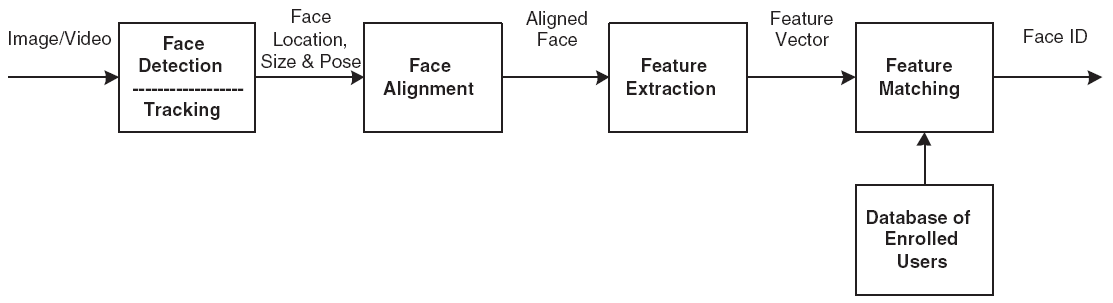
\includegraphics[width=\textwidth]{img/8_1.png}
    \caption{Face recognition processing flow}
    \label{fig:8_1}
\end{figure}

Face detection finds the face areas in the input image. If the input is a video, to be more efficient and also to achieve better robustness, face detection is only performed on key frames and a tracking algorithm is applied on interval frames. Face alignment is very similar to detection, but it is aimed at achieving a more accurate localization. In this step, a set of facial landmarks (facial components), such as eyes, brows and nose, or the facial contour are located; based on that, the face image is rotated, chopped, resized and even warped, this is called geometrical normalization. Usually the face is further normalized with respect to photometrical properties such as illumination and gray scale.

Feature extraction is performed on a normalized face to provide effective information that should be useful for recognizing and classifying labels in which there is interest, such as identity, gender, or expression. The extracted feature vector is sent to a classifier and compared with the training data to produce a recognition output.

\section{Face Detection}
Face detection is the first step in face recognition. It has a major influence on the performance of the entire system. Several cues can be used for face detection, for example, skin color, motion (for videos), facial/head shape, and facial appearance. Most successful face detection algorithms are based on only appearance. This may be because 

Pg 9-14

Saket:- Add 15-16 by Shweta
Saket:- Add 17-18 by Shelke

Rohit:- Add Swapnil, You and Kadam
\end{document}